Nick Vosseteig

2014-12-5

building, wiring, programming

\begin{tabular}{|p{5cm}|p{5cm}|}
 \hline
 building&
This week we replaced the cardboard with plastic on the launcher and built a part to grab the base of the tubes.
 \\
 \hline
wiring&
Alex and I worked on the wiring and soldered the wires to the motors.
 \\
 \hline
programming&
Updated the code and changed controller configuration.
 \\
 \hline
\end{tabular}

\section*{building}
We built a grabber on the back of the robot to grab onto the base of the tube and drag it with us. We also replaced the main launcher with a plastic counterpart so that it is stronger, hits the ball with more force, and doesnt break very easily.
\section*{Wiring}
We fixed up the wiring some more and soldered the wires to the motors to make them stay on better and to save space.

Here is a picture of me soldering the wires to the motor:
\begin{center}
 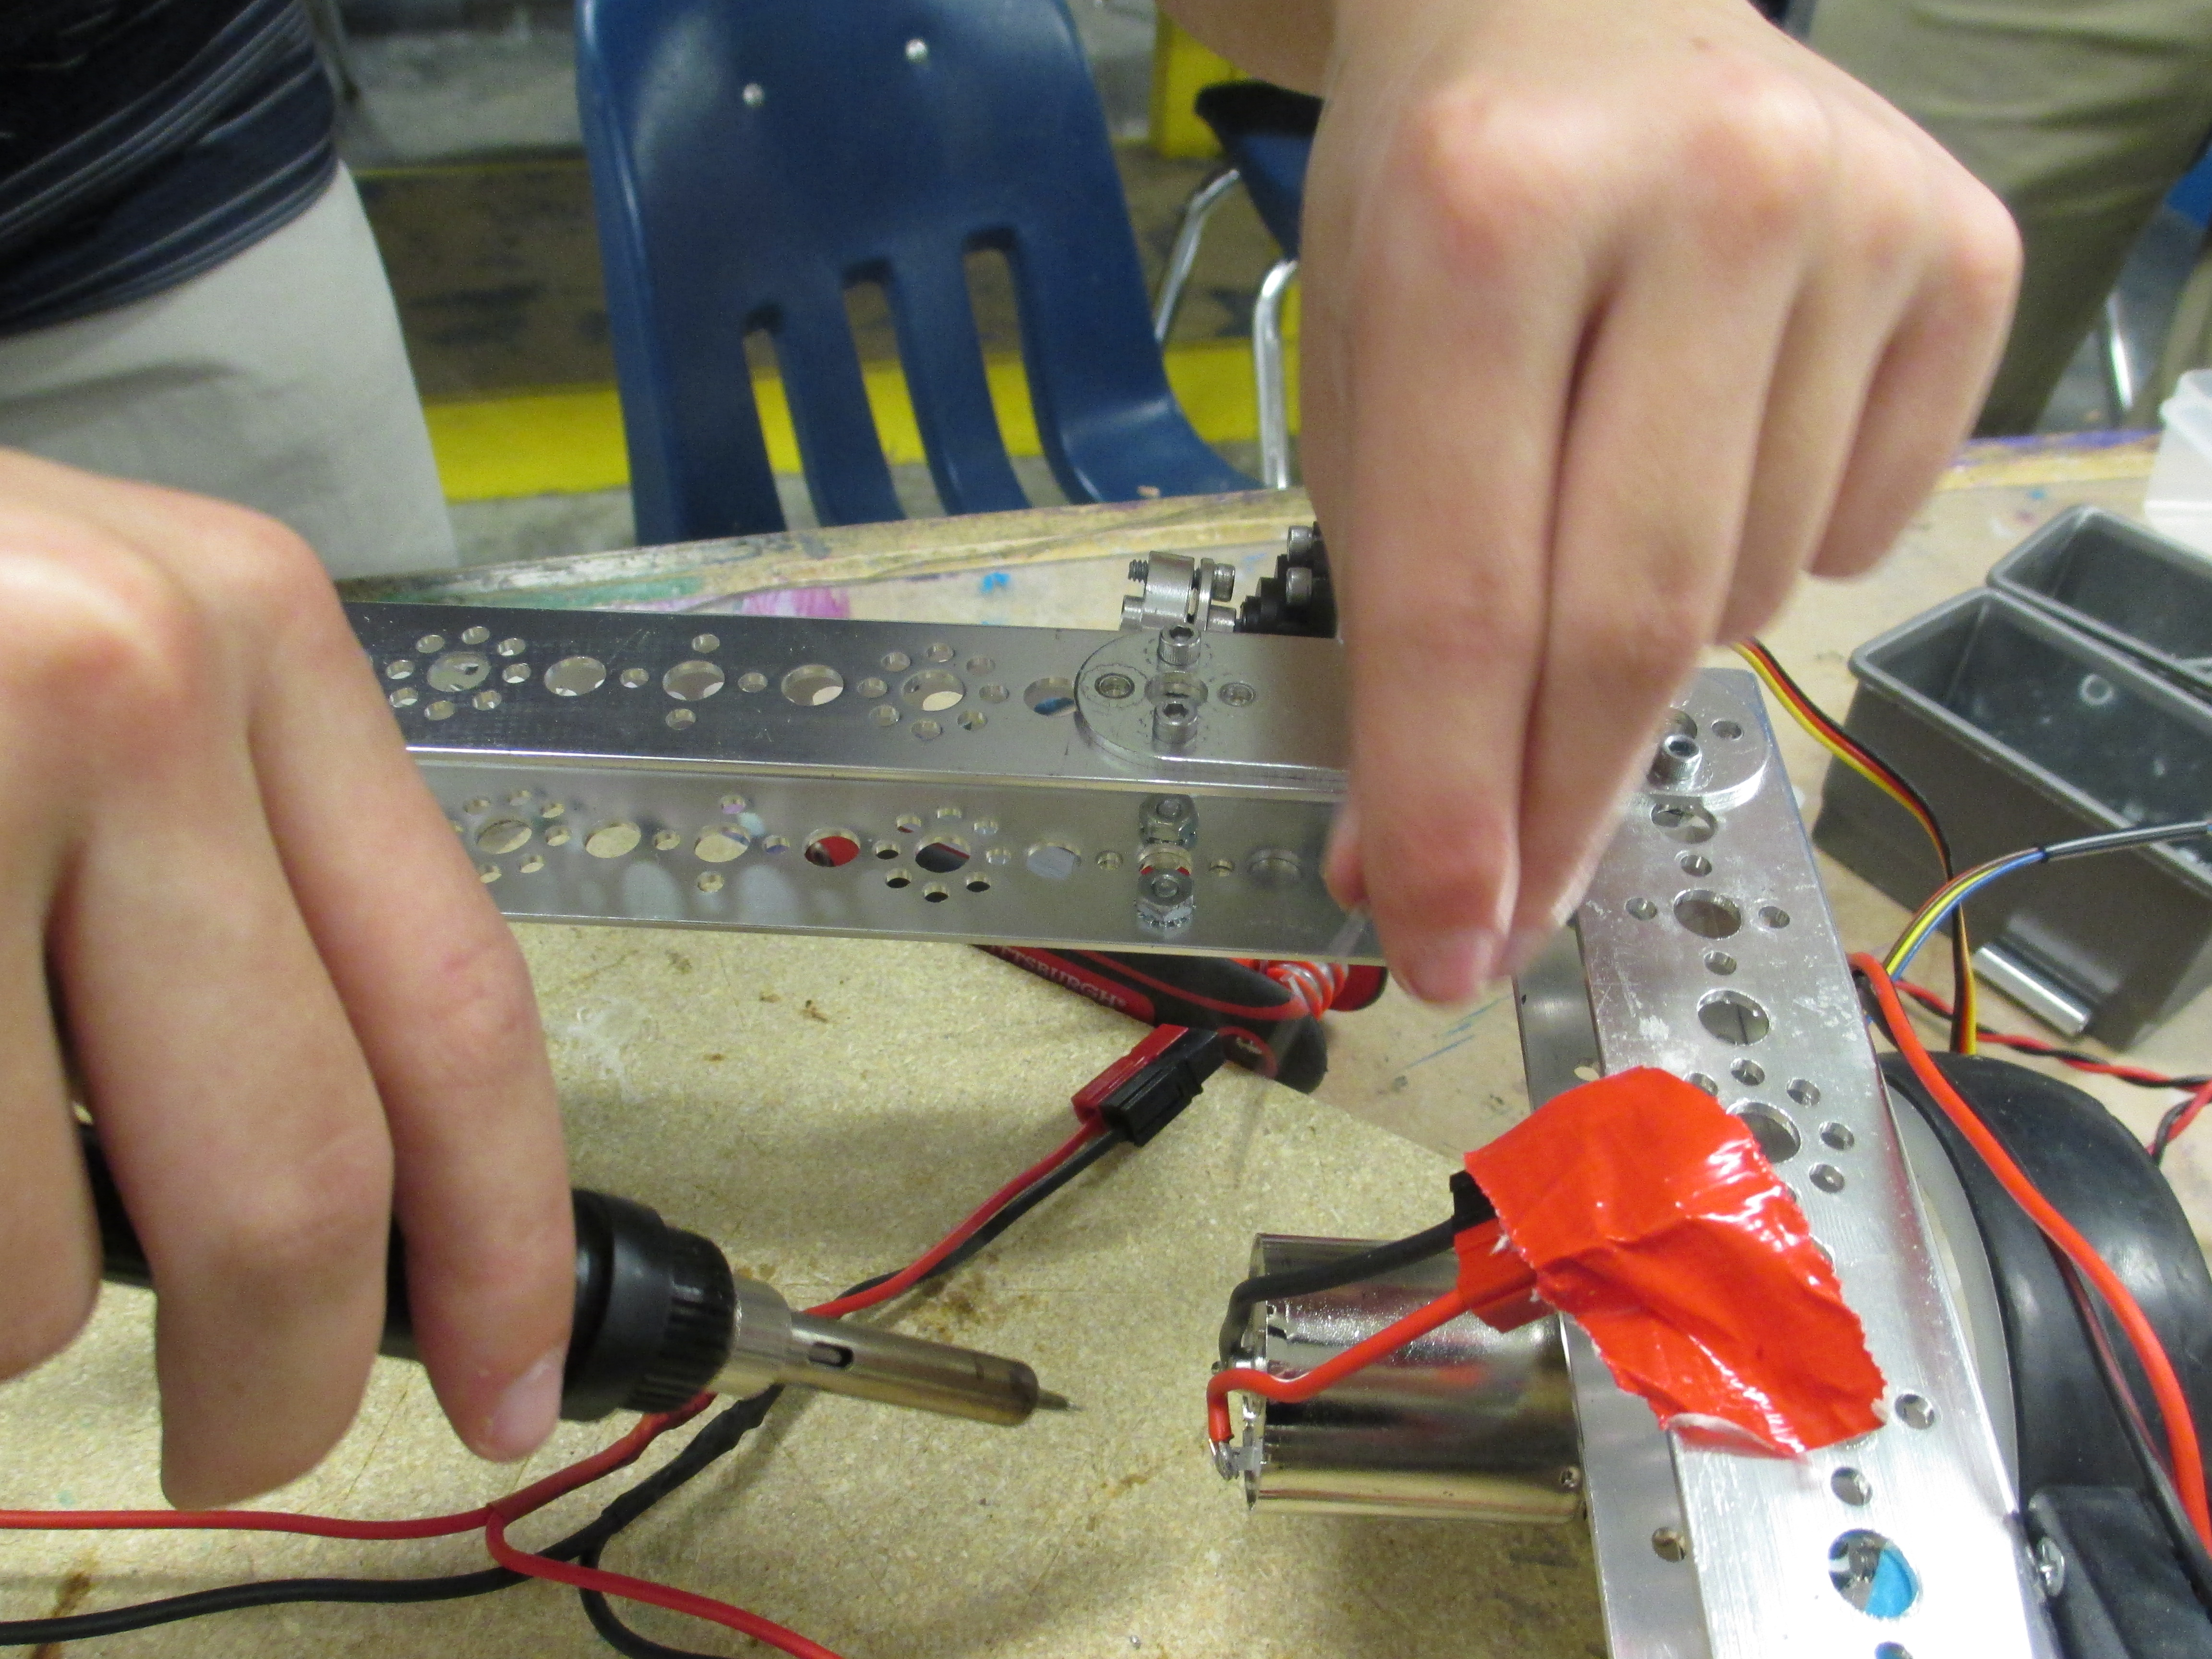
\includegraphics[width=215px]{./Entries/Images/nick_soldering.jpg}
\end{center}